\documentclass[fleqn]{jbook}
\usepackage{physpub}

\begin{document}

\begin{question}{教育 物理}{}

\begin{subquestions}
\SubQuestion
電荷$+Ze$を持つ非常に重い原子核に向かって、質量$m$、電荷の$q$の荷電粒子が初速度$v_0$
を持って無限遠から衝突パラメータ$($ 無限遠での粒子の運動方向を延長して得られる直線と標的
$($ ここでは原子核 $)$ との距離 $)$ $b$ で近づくとき、次の問いに答えよ。
ただし、粒子間にはクーロン力のみが働くものとし、原子核の反跳は無視する。
また、クーロンの法則の比例定数は$k$とせよ。\\
\begin{center}
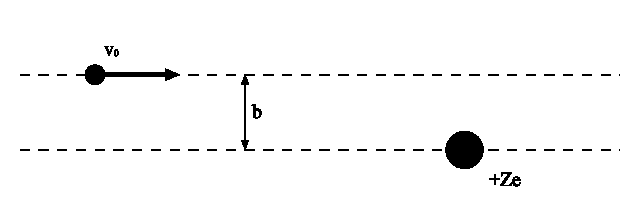
\includegraphics[clip,height=4cm]{1998phys1-1.eps}
\end{center}


\begin{subsubquestions}
\SubSubQuestion
 荷電粒子の描く軌道を、衝突パラメータ$b$が大きい場合と小さい場合 $($ ただし$b>0$ $)$、
 および$q$の符号が正と負の場合、計四つの組み合わせについて、同一の図の中に定性的に描け。

\SubSubQuestion
荷電粒子が持つ原子核の周りの角運動量$\vec{L}$を、原子核を原点とする荷電粒子の位置ベクトル$\vec{r}$を用いて表わせ。

\SubSubQuestion
$\vec{L}$が保存することを示せ。

\SubSubQuestion
衝突パラメータが$b$であるとき、$\vec{L}$の大きさを求めよ。

\SubSubQuestion
軌道上で荷電粒子が原子核に最も近づく点における粒子間の距離を$s$とするとき、
この点における荷電粒子の速さ$v_{s}$はどう表わされるか。

\SubSubQuestion
$q=+e$とするとき、$s$を求めよ。

\end{subsubquestions}


\SubQuestion
半径$a$の球内に電荷が一様に分布している。球の外側には電荷はないものとする。
球内の電荷分布を$\rho ( >0 )$として、以下の問いに答えよ。
\begin{subsubquestions}
\SubSubQuestion
球の内外の電場の大きさ $E(r)$ を、球の中心からの距離$r$の関数として求め、そのグラフを描け。

\SubSubQuestion
同じく球の内外の静電ポテンシャル$\phi(r)$を$r$の関数として求め、そのグラフを描け。
ただし、無限遠での静電ポテンシャルを$0$とすること。

\SubSubQuestion
 無限遠から少しずつ電荷を持ってきてこのような電荷分布をつくるのに要する仕事$W_{1}$を計算せよ。

\SubSubQuestion
球内および球外の空間の静電場のエネルギーをそれぞれ計算し、全空間の静電場のエネルギー$W_{2}$を求めよ。
\end{subsubquestions}

\SubQuestion

媒質中を伝播する音は、媒質の密度の波である。
$\Delta \rho $ を平均密度$\rho$ からのずれとすると、
$x$方向に伝播する音波は、波動方程式
\[
k\frac{\partial^{2}(\Delta \rho)}{\partial x^{2}}
=\frac{\partial^{2}(\Delta \rho)}{\partial t^{2}}
\]
に従う。
ここで$k$は、断熱過程での$\rho$に対する圧力$P$の変化率
\[
k=\left.\frac{dP}{d\rho}\right|_{adiabatic}
\]
である。
媒質が、温度の$T$理想気体である場合について、以下の問いに答えよ。
ただし、理想気体の分子量を$M$、定積比熱に対する定圧比熱の比を$\gamma$、気体定数を$R$とする。

\begin{subsubquestions}
\SubSubQuestion
理想気体の圧力$P$が、$P=\rho R T /M$と表されることを示せ。

\SubSubQuestion
$k$を、$M$、$\gamma$、$T$および$R$を用いて表せ。ただし、断熱過程では、$P/\rho^{\gamma}=$一定であることを用いてよい。

\SubSubQuestion
ヘリウムガス($M=4.0,\gamma=5/3$)中の音速は、
同じ温度の窒素ガス($M=28.0,\gamma=7/5$)中の音速の何倍になるか、有効数字2桁で答えよ。

\SubSubQuestion
理想気体中に、片端を閉じ他端を開いた長さ$l$の管をおく。
管の中の気柱にたつ音の基本定在波の振動数$\nu_{0}$を、音速を$v$として、求めよ。
それに基づいて、ヘリウムガス中と窒素ガス中での$\nu_{0}$の違いを簡潔に説明せよ。

\SubSubQuestion
同じ温度のヘリウムガスと窒素ガスが、図のように薄膜で隔てられているとき、ヘリウムガス中から斜めに入射した音波はどのように進むか、図示し簡潔に説明せよ。\\

\begin{center}
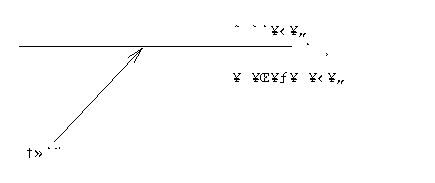
\includegraphics[clip,height=4cm]{1998phys-3.eps}
\end{center}

\end{subsubquestions}
\end{subquestions}
\end{question}
\begin{answer}{教育 物理}{}

\begin{subanswers}
\SubAnswer

\begin{subsubanswers}
\SubSubAnswer
力は $ \frac{kZeq}{r^{2}} \frac{\vec{r}}{r}$ 
( $ \vec{r}$は原子核から荷電粒子の方向)で、$ r^{2} $が小さいほど力は強いことに注意すると、\\

\begin{center}
\includegraphics[clip,height=4cm]{1998phys1-2.eps}
\end{center}


\SubSubAnswer
$ \vec{L}=\vec{r}\times \vec{p} $なので、
$ \vec{L}=m\vec{r}\times \vec{v}=m\vec{r}\times \vec{\dot{r}} $。


ちなみに、 $\vec{r}$ と$\vec{v}$の関係を求めておくと、
荷電粒子の全エネルギーは、$\frac{1}{2}mv^{2}+k\frac{Zeq}{r}$なので、エネルギーの保存より、
\begin{eqnarray}
\frac{1}{2}mv_{0}^{2}&=&\frac{1}{2}mv^{2}+k\frac{Zeq}{r} \nonumber \\
v^{2}&=&v_{0}^{2}-\frac{Z2eqk}{mr} \eqname{Q1}
\end{eqnarray}


\SubSubAnswer
$\vec{L} $ を時間微分すると、
\[
\frac{d\vec{L}}{dt}
=\frac{d}{dt}(m\vec{r}\times \vec{\dot{r}})
=m( \vec{\dot{r}}\times \vec{\dot{r}}
        +\vec{r}\times \vec{\ddot{r}} )
=m(\vec{r}\times \vec{\ddot{r}})
\]
 運動方程式
$ m\vec{\ddot{r}}=\frac{kZeq}{r^{2}}\frac{\vec{r}}{r} $
を使うと、これは0になる。よって示された。


\SubSubAnswer
$|\vec{L}|$を求める。
保存するので、無限遠で求めればよい。 
\[
|\vec{L}| =m|\vec{r}\times \vec{\dot{r}}| =m|\vec{r}\times \vec{v_{0}}| = mbv_{0}.
\]


\SubSubAnswer
一番近づいた時、$\vec{v} \bot \vec{r}$。
よって、$|\vec{L}| = msv_{s}=mv_{0}$より、$v_{s}=v_{0}\frac{b}{s}$。


\SubSubAnswer
\eqhref{Q1}より、$v_{s}^{2}=v_{0}^{2}-\frac{2Ze^{2}k}{ms}$ 
よって、
\begin{align*}
&\frac{v_{0}^{2} b^{2}}{s^{2} }=v_{0}^{2}-\frac{2Ze^{2}k}{ms}\\
&s^{2}-\frac{2Ze^{2}k}{mv_{0}^{2}}s-b^{2}=0\\
&s=\frac{Ze^{2}k}{mv_{0}^{2}}\pm\sqrt{\frac{Z^{2}e^{4}k^{2}}{m^{2}v_{0}^{4}} + b^{2}}.
\end{align*}
$s>0$なので、+の方が答。

\end{subsubanswers}

\SubAnswer
\begin{subsubanswers}

\SubSubAnswer
電荷分布が球対称なので、電場も球対称。
\begin{itemize}
\item $r>a$ のとき。Gaussの法則より、
\begin{eqnarray*}
	\int E(r) dS = 4\pi r^{2} E(r) &=& \frac{1}{\varepsilon_{0}}\frac{4\pi}{3}a^{3}\rho \\
	E(r)&=&\frac{a^{3}\rho}{3\varepsilon _{0} r^{2}}.
\end{eqnarray*}
\item $r<a$ のとき。内部電荷は\(\frac{4\pi}{3}r^{3}\rho \)より、
\begin{eqnarray*}
	\int E(r) dS = 4\pi r^{2} E(r) &=& \frac{1}{\varepsilon_{0}}\frac{4\pi r^3}{3}\rho \\
	E(r)&=&\frac{\rho}{3\varepsilon _{0}} r.
\end{eqnarray*}	
\end{itemize}
よって、グラフにすると、\\
\begin{center}
\includegraphics[clip,height=4cm]{1998phys2-1.eps}
\end{center}

\SubSubAnswer
$\vec{E}=-\nabla \phi$ より、
$\phi = -\int \vec{E}\cdot d\vec{r}=-\int E(r)dr$
なので、

$r>a$では、
\[
\phi(r)=-\int \frac{a^{3}\rho}{3\varepsilon_{0}}\frac{1}{r^{2}}dr
=\frac{a^{3}\rho}{3\varepsilon_{0}} \frac{1}{r} + A.
\]
$r\rightarrow \infty$で、$\phi\rightarrow 0$より、$A=0$。
よって、$\phi(r)=\frac{a^{3}\rho}{3\varepsilon_{0}} \frac{1}{r}$.

$r<a$では、
\[
\phi(r)=-\int \frac{\rho}{3\varepsilon_{0}}rdr
=-\frac{\rho}{6\varepsilon_{0}}r^{2} + B.
\]
$r=a$で連続より、
\begin{eqnarray*}
-\frac{\rho a^{2}}{6\varepsilon_{0}}+B&=&\frac{a^{2}\rho}{3\varepsilon_{0}}\\
B&=&\frac{\rho a^{2}}{2\varepsilon_{0}}.
\end{eqnarray*}
結局、$\phi(r)=-\frac{\rho}{6\varepsilon_{0}} r^{2}+\frac{\rho a^{2}}{2\varepsilon_{0}}$.\\

\begin{center}
\includegraphics[clip,height=4cm]{1998phys2-2.eps}
\end{center}


\SubSubAnswer
微小な電荷を無限遠から何回か運んできた後、
半径$a$の電荷球の電荷密度が$\rho '$になっているとする。
ここで、さらに微小な電荷$\Delta q$を運んでくると、
電荷球の電荷密度が$\Delta \rho = \frac{3}{4\pi a^{3}}\Delta q$だけ増える。
$r \sim r+dr$の微小体積の電荷密度を$\Delta \rho$だけ増すのに必要な仕事は、
\[
\left(-\frac{\rho '}{6\varepsilon_{0}} r^{2} + \frac{a^{2}\rho '}{2\varepsilon_{0}} \right)
4\pi r^{2} \Delta \rho dr.
\]
よって、全球の電荷密度を$\Delta \rho$だけ増すのに必要な仕事$\Delta W$は
\[
\Delta W
=\int_{0}^{a} \left(-\frac{\rho '}{6\varepsilon_{0}} r^{2} + \frac{a^{2}\rho '}{2\varepsilon_{0}} \right)4\pi r^{2} \Delta \rho dr
=\frac{2\pi}{\varepsilon_{0}}\Delta \rho \rho'\frac{4}{15}a^{5}.
\]
したがって、電荷密度を$\rho$にするまでに必要な仕事$W_{1}$は、
\[
W_{1}=\int \Delta W 
= \int_{0}^{\rho} \frac{2\pi}{\varepsilon_{0}}\rho'\frac{4}{15}a^{2}d\rho '
= \frac{4\pi a^{5}}{15\varepsilon_{0}}\rho^{2}. 
\]

\SubSubAnswer
単位体積あたりの静電場のエネルギー$u$は、$u=\frac{1}{2}\varepsilon_{0}E^{2}$。
よって、球内では、
\[
u_{in} = \frac{1}{2}\varepsilon_{0}E^{2}
=\frac{\varepsilon_{0}}{2} \cdot \frac{ \rho^{2} }{ 9\varepsilon_{0}^{2} }r^{2}
=\frac{\rho^{2}}{18 \varepsilon_{0}} r^{2}.
\]
したがって、全部で、
\[
U_{in}=\int \frac{\rho^{2}}{18 \varepsilon_{0}} r^{2} d^{3}r
=4\pi \frac{\rho^{2}}{18 \varepsilon_{0}} \int_{0}^{a} r^{4} d^{3}r
= \frac{2 \pi \rho^{2}}{9 \varepsilon_{0}} \frac{a^{5}}{5}.
\]
球外では、
\[
u_{out} = \frac{1}{2}\varepsilon_{0}E^{2}
=\frac{\varepsilon_{0}}{2} \cdot \frac{ a^{6}\rho^{2} }{ 9\varepsilon_{0}^{2} r^{4}}
=\frac{\rho^{2}}{18 \varepsilon_{0}} \frac{a^{6}}{r^{4}}.
\]
全部で、
\[
U_{out}=\int \frac{\rho^{2}}{18 \varepsilon_{0}} \frac{a^{6}}{r^{4}} d^{3}r
=4\pi \frac{\rho^{2}}{18 \varepsilon_{0}} a^{6}\int_{a}^{\infty} \frac{1}{r^{2}} d^{3}r
= \frac{2 \pi \rho^{2}}{9 \varepsilon_{0}} a^{5}.
\]
以上より、全空間の静電場のエネルギーは、
\[
W_{2}=\frac{2 \pi \rho^{2}}{9 \varepsilon_{0}} a^{5}\left( \frac{1}{5}+1 \right)
=\frac{4 \pi \rho^{2}}{15 \varepsilon_{0}} a^{5}.
\]
\end{subsubanswers}

\SubAnswer
\begin{subsubanswers}
\SubSubAnswer
理想気体の状態方程式は$PV=nRT$で、気体の重さ$m$は$m=nM$より、$n=m/M$で、$PV=mRT/M$。
$\rho = m/V$より、
\begin{equation}
P=\frac{\rho R T}{M}. \eqname{Q4}
\end{equation}


\SubSubAnswer 
\begin{equation}
\frac{P}{\rho^{\gamma}}=C \eqname{Q2}
\end{equation}
より、$P=C\rho^{\gamma}$である。
よって、
\begin{equation}
k=\frac{dP}{d\rho}=C\gamma\rho^{\gamma -1}. \eqname{Q3}
\end{equation}
Cを求める。\eqhref{Q2}に\eqhref{Q4}を代入すると、
\begin{eqnarray*}
\frac{RT}{M}\frac{1}{\rho^{\gamma -1}}&=&C\\
C\rho^{\gamma -1}&=&\frac{RT}{M}.
\end{eqnarray*}
これを\eqhref{Q3}に代入して、$k=RT\gamma /M$


\SubSubAnswer
 音速を$v$とすると、$\Delta \rho = f(x-vt)$とおけて、
$kf''=v^{2}f''$。
よって、$v=\pm \sqrt{k}$。
従って、
ヘリウムガスの音速は$\sqrt{\frac{RT}{4}\frac{5}{3}}$、
窒素ガスの音速は$\sqrt{\frac{RT}{28}\frac{7}{5}}$ なので、
ヘリウムガスの音速は、窒素ガスの音速の
$\sqrt{\frac{5RT}{4\cdot 3}}\cdot \sqrt{\frac{28\cdot 5}{7RT}}\simeq 2.9$倍。

\SubSubAnswer
閉じた方は固定端で開いた方は自由端である。
波長は図から$\lambda_{0}/4=l$で、$\lambda\nu_{0}=v$。
よって、$\nu_{0}=v/\lambda_{0}=v/4l$。
したがって、ヘリウムガスのほうが窒素ガスより振動数が大きくなる。\\
\begin{center}
\includegraphics[clip,height=2cm]{1998phys3-1.eps}
\end{center}

\SubSubAnswer
普通に、速さの速い方から遅い方への入射となる。
角度は屈折の法則より、
$\frac{\sin \theta}{\sin \phi}=\frac{v_{N}}{v_{He}}$となる。

\begin{center}
\includegraphics[clip,height=4cm]{1998phys3-2.eps}
\end{center}

\end{subsubanswers}
\end{subanswers}
\end{answer} 
\end{document}













